% This is "sig-alternate.tex" V1.9 April 2009
% This file should be compiled with V2.4 of "sig-alternate.cls" April 2009
%
% This example file demonstrates the use of the 'sig-alternate.cls'
% V2.4 LaTeX2e document class file. It is for those submitting
% articles to ACM Conference Proceedings WHO DO NOT WISH TO
% STRICTLY ADHERE TO THE SIGS (PUBS-BOARD-ENDORSED) STYLE.
% The 'sig-alternate.cls' file will produce a similar-looking,
% albeit, 'tighter' paper resulting in, invariably, fewer pages.
%
% ----------------------------------------------------------------------------------------------------------------
% This .tex file (and associated .cls V2.4) produces:
%       1) The Permission Statement
%       2) The Conference (location) Info information
%       3) The Copyright Line with ACM data
%       4) NO page numbers
%
% as against the acm_proc_article-sp.cls file which
% DOES NOT produce 1) thru' 3) above.
%
% Using 'sig-alternate.cls' you have control, however, from within
% the source .tex file, over both the CopyrightYear
% (defaulted to 200X) and the ACM Copyright Data
% (defaulted to X-XXXXX-XX-X/XX/XX).
% e.g.
% \CopyrightYear{2007} will cause 2007 to appear in the copyright line.
% \crdata{0-12345-67-8/90/12} will cause 0-12345-67-8/90/12 to appear in the copyright line.
%
% ---------------------------------------------------------------------------------------------------------------
% This .tex source is an example which *does* use
% the .bib file (from which the .bbl file % is produced).
% REMEMBER HOWEVER: After having produced the .bbl file,
% and prior to final submission, you *NEED* to 'insert'
% your .bbl file into your source .tex file so as to provide
% ONE 'self-contained' source file.
%
% ================= IF YOU HAVE QUESTIONS =======================
% Questions regarding the SIGS styles, SIGS policies and
% procedures, Conferences etc. should be sent to
% Adrienne Griscti (griscti@acm.org)
%
% Technical questions _only_ to
% Gerald Murray (murray@hq.acm.org)
% ===============================================================
%
% For tracking purposes - this is V1.9 - April 2009

\documentclass{sig-alternate}
\usepackage{Sweave}

\begin{document}

\title{Course Planning Model}

%\titlenote{(Produces the permission block, and
%copyright information). For use with
%SIG-ALTERNATE.CLS. Supported by ACM.}}
%\subtitle{[Extended Abstract]
%\titlenote{A full version of this paper is available as
%\textit{Author's Guide to Preparing ACM SIG Proceedings Using
%\LaTeX$2_\epsilon$\ and BibTeX} at
%\texttt{www.acm.org/eaddress.htm}}}
%
% You need the command \numberofauthors to handle the 'placement
% and alignment' of the authors beneath the title.
%
% For aesthetic reasons, we recommend 'three authors at a time'
% i.e. three 'name/affiliation blocks' be placed beneath the title.
%
% NOTE: You are NOT restricted in how many 'rows' of
% "name/affiliations" may appear. We just ask that you restrict
% the number of 'columns' to three.
%
% Because of the available 'opening page real-estate'
% we ask you to refrain from putting more than six authors
% (two rows with three columns) beneath the article title.
% More than six makes the first-page appear very cluttered indeed.
%
% Use the \alignauthor commands to handle the names
% and affiliations for an 'aesthetic maximum' of six authors.
% Add names, affiliations, addresses for
% the seventh etc. author(s) as the argument for the
% \additionalauthors command.
% These 'additional authors' will be output/set for you
% without further effort on your part as the last section in
% the body of your article BEFORE References or any Appendices.

\numberofauthors{8} %  in this sample file, there are a *total*
% of EIGHT authors. SIX appear on the 'first-page' (for formatting
% reasons) and the remaining two appear in the \additionalauthors section.
%
\author{
\alignauthor
Luyi Wang\\
       \affaddr{Lane of CSEE Department}\\
       \affaddr{West Virginia University}\\
       \affaddr{Morgantown, West Virginia}\\
       \email{lwang10@mix.wvu.edu}
}
\date{30 July 1999}
% Just remember to make sure that the TOTAL number of authors
% is the number that will appear on the first page PLUS the
% number that will appear in the \additionalauthors section.

\maketitle
\begin{abstract}

This paper proposed an intelligent course planning agent model which is based on {\em Actory} model.{\em Actory} model is a generic agent model which can be applied into diverse fields by enriching with specific domain knowledge. It utilizes BDI \cite{rao1991mra} model as its archetype.  Simulations generated from it are aimed to illustrate real world scenarios where randomness and bias coexist due to undetermined events happening and environment changeableness within specific domain context.  With accumulatively learning and modeling improvement, ideally an actory model would be able to provide people suggestions on principles which can be derived to a comfortable life pattern.  This paper explains a course planning model which is used to assist academic institutes in planning undergraduate level courses.  This model consists of two sub agents. One is life event producer who takes in charge of generating life changing events which mimics the real life happening. The other is Course actor.  It plays an important role in this model where it simulate a real course provider which dispatches exams and gives out grades.  Also this paper illustrate the learning part in this model, which use the keys mechanism to calculate the bias and promote relearning mechanism.  To accumulatively gaining progress in learning mechanism, several loggers have to be implemented in order to gather running time data and transform them into analyzable data format in learning part.  Challenge are met during the learning part since the automatic reloading strategy would interfere  consistence during learning progress. 

\end{abstract}

% A category with the (minimum) three required fields
%A category including the fourth, optional field follows...
\category{D.2.8}{Software Engineering}{Metrics}[complexity measures, performance measures]

\terms{Agent Modelling}

\keywords{Actory mode, course planning}

\section{Introduction}
Course planning is always a challenge issue for academic institutions.  A well defined course planning system would promote the educational quality by arranging course through prerequisite chain. Meanwhile it would relieve student's pressure in confronting with heavy workload and help them build up a systemic knowledge system.  With more and more research carrying on this area, some obvious demands are also brought in. First is the matrix structure of course prerequisite chain.  There is no obviously cut-off line to separate courses according to their easiness levels.  Some high-level theoretical courses are usually build upon rudimental courses which are provided in certain years. A certain number of courses focus more on practice and experiment which asks for  knowledge from both theory and implementation.  Second is how to seek a trade off between the flexibility of timeline and credit hour requirement.  Usually a college level degree requires student get at least 130 credit hours in 4 years.  With these motivation, an course planning system built upon existing academic requirement is required,accompany with adaptive to the dynamic prerequisite chain and flexibilities on course credit hour. \\

This paper proposed an approach to building such a agent technologies based one of BDI agent framework, Actory,  with the domain specific knowledge for course planning.   It utilizes the notion of generic programming and first-order agent language to fulfill above requirements. In section 2,  it introduces some notions of generic programming used in this system and also explains the framework of actory. Section 3 focus on describing the logic view of course planning model and details its implementation. Section 4 gives out the details in model design and the learning mechanism .  The end section, Section 5, concludes current research status and point out the future work. \\

\section{Actory Model and its generic notions}
Agent oriented programming puts much more effect on adapting with dynamic environment changing by acquiring new coming in user requirements\cite{bresciani04}.   The whole system evolution progress  are also divided into separate phrases by specific requirements  according to agent oriented programming notions.  An empirical agent architecture, BDI\cite{rao1991mra} , are widely applied on current agent based system.  It brings in a mature mentalistic notions which helps the developer and users to interpret the logic underneath the agent based system.\\

\subsection{Actory Model}
 \textbf{ Actory Model}, a under developing agent model, also utilize BDI notions to reveal the methodology on domain-specific agent programming level.  This Model consists of three components: Factory, Machine and Transitions and system actor \cite{Levesque94golog:a}. 
 The system actor, called App, is introduced to control the whole work flow in the system. The component Factory plays an important roles in the system as a coordinator who gather all kind of resources and allocate them according to dynamic requirement from machines. Machine itself is regarded as an interactive agent who can dynamically load transitions who takes charge of fulfills task and communicates between machines.  Fig.1 is the basic Architecture of Actory Model. \\

\begin{figure}[h]
\centering
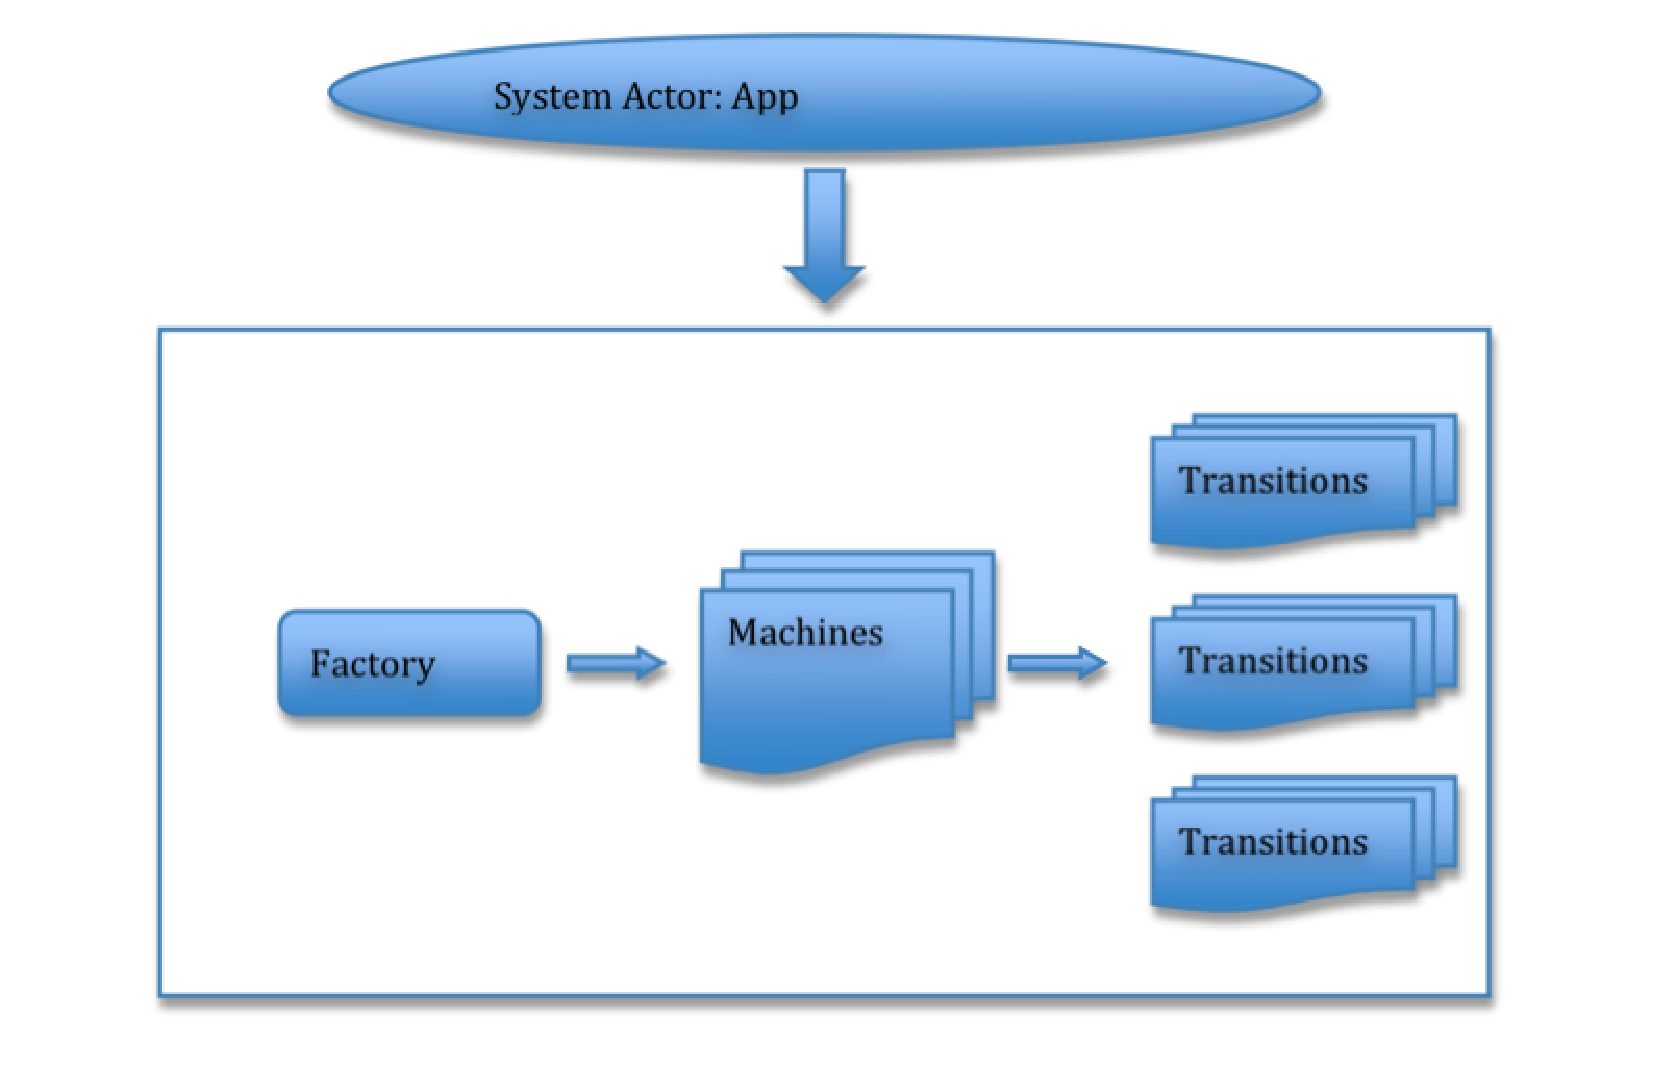
\includegraphics[width=90mm ]{actorymodel}
\caption{Actory Model Structure}
\end{figure}

Based on above architecture, we can see the logic underneath the system is quite obvious with one to many mapping, wherever one factory can contains more than one machines while machine can hold up at least one transitions.  To solve the resource conflicts and reach the concurrency requirement, a semaphore named "asynchronous" is introduced into "App" system actor.  Moreover, this structure provides a framework for enriching with domain specific knowledge without caring environments. Specific domain level programming can be derived from upper level as factory or machine as sub-agent. Meanwhile, tasks on specific domains are implemented as transitions which are gathered and submitted to the domain factory through domain machines. 
\subsection{Generic Notions}
As we discussed in the actory model, we can see several notions, such as factory, machines,etc, are essential in defining the BDI architecture for this model.  Before we proceed to give out the detail notions, we first examine the structure of this components.  The factory component contains one factor called {\em patience} which is controlled by the system actor app.  When the factory loses its temper, or the system actor app reach its limits, defined as {\em toomuchloops},  the system  is terminated.   To this point, we can regard the system's final belief as keep patience and keep running for fulfilling all tasks.  Correspondingly,  the machine component has several constraints on state checking, which is related to the transition component.  The transition component states the adaptation of environment by bringing in condition examine an switching.  The {\em guard} condition determines what the {\em next} state is, and  meanwhile {\em sideeffect} controls the system status changing, such as push hard to lose patience.   So here we can see the desire in actory is trying to keep the patience as many as possible and intention is to fulfill the task by switching to {\em normal state} instead of to {\em loop state }or {\em error state}.   So till here, we can use the Table 1. to illustrate the logic view underneath the system.
\begin{table}[h]
\centering
\caption{BDI notions in Actory Model}
\begin{tabular}{|c|c|c|}\hline
Component Name & BDI Notions & Factor Name \\
\hline
Factory & Belief & Patience\\
\hline
Machine & Desire & Start \\
\hline
Transition & Intention & Next,Guard, SideEffect \\
\hline
\end{tabular}
\end{table}

\section{Course Planning Domain Specific Model}
As we narrated before, course planning is an essential part in academic education.  Based on actory model, we can simulate a virtual college environment in which students take courses and enjoy their college life by participate event like football game.  This is also the feature of actory model, domain specific programming.  \\

\subsection{CP Model Structure}
To enrich actory with domain specific feature, we have to derived component from actory model and brings in sub-system actor which acts as a coordinator in resource allocation and communication. Here we derived two classes from {\em Machine} component as {\em Course} and {\em Student}.    To generate tasks for these two new components, we invented two sub-system actors as {\em CourseEvent} and {\em LifeEvent}, respectively creating events for course and student life.  Fig 2. Show the Course Planning Model Structure after introducing more components.\\

\begin{figure}[!h]
\centering
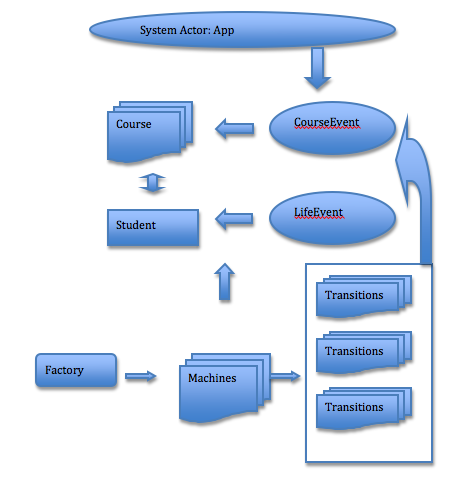
\includegraphics[height=3.5in, width =3.5in ]{courseplanmodel}
\caption{Course Planning Model Structure}
\end{figure}

\subsection{CP BDI Notions}
These two sub-system actors still use the patience to control their work flow and termination state.  So this model stills use actory BDI mentalism.  For the student component, we bring in one factor called {\em happiness} to extend its belief.  So from a student perspective, he/she would like to live with happiness and without losing their temper.  To reach this point, they need to seek a balance between life and academic workload.   But this structure doesn't affect the original BDI mentalism established in the actory model. Table 2 gives out the extended BDI architecture in course planning model.\\
\begin{table*}
\centering
\caption{BDI notions in Course Planning Model}
\begin{tabular}{|l|l|l|l|}\hline
Component Name & Derived Componet & BDI Notions & Factor Name \\
\hline
App & Object & System Actor & Patience\\
\hline
CourseEvent, LifeEvent & App & Sub-system Actor & Patience\\
\hline
Factory & Factory  & Belief & Patience\\
\hline
Student, Course & Machine & Desire & Patience, Happiness \\
\hline
Transition& Transition & Intention & Next,Guard, SideEffect \\
\hline

\end{tabular}
\end{table*}

\subsection{CP Work Mechanism}
In this course plan model, student actively choose courses which is disordered.  Correspondingly, subsystem actor, {\em Lifeevent}, would dynamically generate life events while another {\em courseevent} is generating course events for the course the student taken.  The factor {\em happiness} defined in the student component determines the number of events the student can hold.  When some positive activities, such as {\em win lottery}, take place, the happiness value would be raised up.  Oppositely, the negative activity would reduce the happiness value, such as getting bad grades for exam.  When the events generated, the system actor patience is losing till it enters its termination states where we defined as patience value to 0. Current design doesn't allow the patience value to increase which would lead to an endless state. Also to prevent this happen, a factor called index is introduced in subsystem factor to control the maximum event number which is set as 50.\\

Also as we stressed before, the Course Plan Model should conquer challenges of course matrix prerequisite chain.  In this course plan model,  each course has its corresponding prerequisite chain which can be looked up. An already taken course would relieve patience of sub-system actor,{\em course event}, to deduct the number of events which is generated automatically.  This is fair in real life situation.  Also this mechanism would solve the matrix problem by indexing courses, which is currently not implemented. \\ 

\section{Other Component Design}
\subsection {Automaton component}
As we illustrated above, the components and actors are implemented as machine and App respectively. Except these components, we also implemented several automaton component to provide fundamental support for these components.  Table 3 gives out their name and its functionalities. 

\begin{table}[h]
\centering
\caption{Automaton Components  }
\begin{tabular}{|c|c|}\hline
Component name & functionality  \\
\hline
StudentState & providing transition state.\\
\hline
Guard & providing certain guard\\
\hline
SideEffect & provide certain side effect\\
\hline
\end{tabular}
\end{table}
3
In order to understand how the automaton machine works, we need to first examine the transition structure. \\
\begin{equation}
Trans(X)= (Guard)?(Curr\_St ):(N\_St, [SE]). 
\end{equation}

where $Curr\_St$ denotes Machines X's current state, $N\_st$ is its next state when certain $Guard$ is satisfied.  $SE$ is a side effect which would affect the running environment while the transition fires.  \\

In Course Planning model, the transitions are regarded as events taking place in daily life, such as {\em football} event indicating student is going to watch a football game.  This transition would change the student's state, such as from {\em work state} to {\em happy state} for {\em football} instance.  Also certain side effect would correspondingly occurs, such as increase student's happiness once switching to {\em happy} state.   These domain specific features should be periodically added into while we are gaining much more knowledge of a domain.  Also result is hard to predicted or predefined prior to the event generated.  All these call for us to implement these functionalities into automaton machines. For example, the {\em "student state"} automaton machine would pop out state from states dictionary where stores states predefined or accumulatively added.  Every thing has two sides, the flexibility brought by automaton machine also increase the uncertainty in learning mechanism, such as switching from certain state to another state wouldn't trigger the same side effect. Sometimes it is unreasonable in real life such as winning game won't excite you but make you feel sad.  However this the fault of automaton machine. \\

\subsection {Logger Component}
In order to implement learning, each transition fire should be recorded by a logger in a traceable history.   in Course Planning model, two type of logger are introduced.  First is factory level logger which recorded all activities happened within this domain.  This is also fulfill the requirement of Agent Protocol Message part, rectified in FIPA 1998 agent standard\cite{FIPA1998}. Second one is a {\em stagger} level logger. In actory model, {\em Stagger} works as the basic learning container in which transitions can be shuffled and fixed in certain order.  The logger works on this level is responsible to register transitions and record their fire history.   These two logger components construct a full model logger.  When a transition is generated, it is registered into his container, a stagger belongs to certain machine.  When this machine enters a factory, all its transitions are registered into the corresponding factory logger.  Obviously,  when a machine leaves the factory, a factory logger won't record this machine's activities any more, but still provides logger service for other machines residing in itself.  The activities of transitions residing in the leaving machines are still recorded through the stagger logger belonging to the machine.  This is reasonable and won't miss out any activities in the model.  In the learning part, we may examine this structure, some deeper analysis is provided. 

\begin{table}[h]
\centering
\caption{Logger Components  }
\begin{tabular}{|c|c|}\hline
Component name & functionality  \\
\hline
FactoryLogger & log all activities residing in factory\\
\hline
StaggerLogger & log all activities residing in stagger\\
\hline

\end{tabular}
\end{table}



\subsection{Stagger and Stagger logger}
Stagger works as an essential part in actory model.  Basically almost all the active components use stagger as its container. For example, active {\em machines} residing in  a factory are putted into a stagger; transitions residing in a machine are putted into a stagger.  We can regarded the stagger contains the activities in the actory model so that a stagger should provide functionalities to control these activities. The basic control enforced here is shuffle and fix.  Shuffle rearranges the activity order, which would affect their fire order. Fix also rearrange the activity order but certain activity is fixed into certain location and others are still shuffled. This control mechanism is used in learning part.   To facilitate control, the stagger logger need to record the activities, analyze it and also choose the control method. 

\section{Course Plan Design}
First we need to know this point, Actory is a model which is used to mimic the real life situation but it is not a real life situation.  Till this point, the learning in Course Planning model is performed upon the simulation used to mimic the real course planning situation.  

\subsection {The Heaven in CP}
In real life, the student is a important role in course planning. The course plan is designed to benifit student more instead of others.  So the scale we used in course planning to evaluate should be upon student. From this view, we can think of a student's life.  A student select course, attend the course.  The course leaves homework, give out exams to student.  The student also have life activities such as watching football,  bidding on ebay.  So a good scale should cover all these aspects.  Nothing can be better than a mental status of student to describe these. So here the scale to evaluate the model we selected is student's happiness.   Activities happened upon student would make him/her happy, sad, calm.  These mental status are also reflected by student's temper. Always doing repeated work would make student lose temper, even a happy one.  So a scale used to control the whole model here is patience. In summary,  two scales, happiness and patience, are the heaven in course planning model. 

\subsection {Working process in CP}
Learning in actory is conducted through logger as we illustrated above.  Before we proceed to understand the learning strategy, we need to go through the working steps in our Course Model simulation. 

\begin{itemize}
\item certain event producer generate events 
\item certain consumer(Student, Course) loads these events.
\item Student works in its mimic real life
\item Student takes courses.  
\item Student participate life activities.
\item Student walk away from its mimic real life. 
\end{itemize}

This simulation process can be explained in actory model language.  A plenty of transitions are generated by CourseEvent and LifeEvent actors. These two subsystem actors start to control which agent should work on these transitions.  Once the agent is selected, the agent starts to load all these transitions into their staggers.  Till these done,  the system actor start to run all agents that all agents start to consume these transitions which would affect temper and happiness. When temper is out, the agent works away from the factory.  The factory is running until all the agents finish their job. 

\section{ Learning in CP}
 Before we show the learning, we should first define the initial value used in this model as table 5 shows.
 
\begin{table}[h]
\centering
\caption{Initial value in CP Model }
\begin{tabular}{|c|c|c|}\hline
Factor name & Component Name & Initial Value \\
\hline
patience & SubS,System Factors & 100\\
\hline
happiness & Student &100\\
\hline
event index & subsystem Factory &50\\
\hline
\end{tabular}
\end{table}

\subsection{Learning design}
From our work process, we can see that a event is generated by the automaton agent which fulfill the requirement on randomness. Meanwhile events are provided by different producer, which enrich them with their specific feature. When they are loaded into machine,machine becomes to share this feature. The only thing without any specific meaning is the factory itself.  If we regard the factory as a space, different machine as the region in this space, and transitions are item in this region. The the whole model is a complete block design.  If we let factory runs certain number times that should be equivalent to the quantity of treatment number $\times$ block number, then this becomes to be a randomized complete block design\cite{statbok}.  At very beginning, all what we concern is randomization so that there is only one treatment.  With the learning goes on, the treatment number would increase since we are going to apply the fixed number of transitions, then the running time also need to increase. 

\subsection{evaluation mechanism and Keys2}
After the event producer provides the events which are generated by automaton agent, their event id is specified. Correspondingly a table used to record all the activities is initialized with rows as each run of factory and column as transition fires in runs.  The factory logger takes the responsibility to fulfill the table with the final happiness and how many transitions fire in it.  The stagger logger is used to record which transition residing it is fired during this run.  The table is looked like Table 6 which contains 6 transitions in 5 runs. 

\begin{table}[h]
\centering
\caption{Transition fire table }
\begin{tabular}{|c|c|c|c|c|c|c|c|}\hline
run no.& t1 & t2 & t3 & t4 & t5 &t6 &final happiness \\
\hline
r1&0&0&0&0&0&0& 100\\
\hline
r2&0&0&0&1&0&0& 120\\
\hline
r3&0&0&1&0&0&0& 88\\
\hline
r4&0&1&0&0&2&0& 144\\
\hline
r5&3&0&0&0&1&1& 40\\
\hline
\end{tabular}
\end{table}

Based on the final happiness value in this table, we can divided the table into two part, best table and rest table, according to certain predefined $\alpha$ value, such as 0.8. So we regard the The best table is a 20\% in total which overwhelmed the other 80\% part of all.  For the above example, the fire table is transformed into following.
 \begin{table}[h]
\centering
\caption{Transformed transition fire table }
\begin{tabular}{|c|c|c|c|c|c|c|c|c|}\hline
run no.&t1 & t2 & t3 & t4 & t5 &t6 &final happiness &label\\
\hline
r1&0&0&0&0&0&0& 100&rest\\
\hline
r2&0&0&0&1&0&0& 120&rest\\
\hline
r3&0&0&1&0&0&0& 88& rest\\
\hline
r4&0&1&0&0&2&0& 144&best\\
\hline
r5&3&0&0&0&1&1& 40&rest\\
\hline
\end{tabular}
\end{table}

When we finish this work, we are going to apply mining mechanism upon it.  Looking at this table, can we conclude the t5 would contribute more for the final happiness? The answer is not sure, we should examine it since comparing with run 2, if the t4 fires twice maybe it would be over r4.  If we can explore out certain set of transitions which would highly improve the performance, then we regards this set is a key set.  So based on this ideal situation, the transitions residing in this set should have a high condense which means it should not spread all cross the space.  So we need to figure out a way to finding them.  This is the keys2 algorithm. \cite{gay09keys}.  The assumption of keys2 is as described above. This problem is similar as clustering problem, where condensed set should be be clustered. K-Mean \cite{kmean} is frequently used and its variance approached is examined by many researcher to achieve higher performance.  This is also should be a research goal towards by our actory model. \\

The measure metric defined in keys2 follows the bayes theorem:
\begin{equation*}
P(H|E) = \frac{P(E|H) * P(H) }{P(E)}
\end{equation*}
Where H here is a set, {\em \{best rest\}} and $E$ is certain transition.  $P(H)$ is $\alpha$ or $1- \alpha$. 
 We can conclude this equation into format:
 \begin{equation*}
 P(H|E)*Support(H|E) = \frac{like(best|E)}{like(rest | E)+ like(best|E)}
 \end{equation*}
Here if we want to examine the {\em likelihood} of t5, we have to follow certain steps. 
\begin{eqnarray*}
\because \alpha =0.8.  \\
\therefore P(best) = 0.2,\\
 p(rest) = 0.8.\\
\because
total\_transitions\_fires\_no =10,\\
total\_transitions\_fires\_no\_in\_best =3.\\
total\_transitions\_fires\_no\_in\_rest =7.\\
t5\_fires\_no=3\\
t5\_fires\_no\_in\_best=2\\
t5\_fires\_no\_in\_rest=1\\
\therefore
freq(t5| best) = 2/3\\
freq(t5 |rest) = 1/7\\
like(best | t5) = freq (t5 | best) * p(best) = 2/3 * 0.2 = 4/30.\\
like(rest | t5) = freq( t5 |rest) * p(rest) = 1/7 * 0.8 = 8/ 70. \\
p(best| t5) = \frac{like(best|t5)}{ like (best | t5) + like( rest | t5)} = 0.53.
\end{eqnarray*}

Since the bayes is usually week in ranking part, keys2 facilitate it with a support factor,$support(H|E)$. The support factor strength the power of best and meanwhile decrease the variance of best. So the final equation is 
\begin{equation*}
P(H|E)*Support(H|E) = \frac{like(best|E)^2}{like(rest | E)+ like(best|E)}
\end{equation*}

For above example, the final result would be 
\begin{equation*}
p(best| t5) = \frac{like(best|t5)^2}{ like (best | t5) + like( rest | t5)} = 0.062
\end{equation*}.

The above process need to be applied on each transition produced by event producer.   There is only one exception in course planning model, the {\em start transition}. In actory model,  the start transition is always fired.  It may or may not contribute the final happiness. However its fixed fire order may cause a effect called carry over effect \cite{} which might affect randomness feature of experiment design. So in course plan simulation, this kind of transitions are eliminated into consideration.  Based on the rank of the transitions, the factory logger would select  a certain small number set of transitions as {\em key transitions} and fixed them.  Other transitions are still be arranged in shuffle.  This would introduce the bias into experiment. To eliminate this, we regarded them into different treatments.  So this won't affect the fairness. The only thing we need to do is increase running time.  So the transition fire table would increase and also computation time would increase.  Theoretically, this is reasonable, since we are confine certain transitions into small set so we have to increase the space range.  If we want to keep space in equivalent,  we have to reduce the total number of transitions.   This is also need to examined into later on research. 
\section{Experimental Result and analysis}
\subsection{ Running Environment}
In term of faireness, the running experiment is conducted on two machines. One box with a Intel 2.26G Hz core processor and 2G DDR3 physical memory and the other is csee.wvu.edu server. The later one is a cluster consisting of multiple linux machines. The machine running this experiment is loaded with a 2.4G AMD core processor with 5G DDR2 physical memory.  
The average running time for 10 times on each machines are listed in Table ~\ref{timetable}.
\begin{table}[h]
\centering
\caption{running time table}
\label{timetable}
\begin{tabular}{|c||c|c|}
\hline
time & macmachine & linuxmachine\\
\hline
real & 4.111&1.463 \\
\hline
user&1.226&0.914\\
\hline
sys & 0.516&0.246\\
\hline
\end{tabular}
\end{table}
\subsection{Running result}
The main purpose of learning is to improve the performance. From the course planning model perspective, it is aimed to help student to construct a systemic learning style in which certain action would help them relief their pressure but also gain performance in learning.  Due to this reason, as we illustrate above, certain transitions are selected based on their keys result. After they are fixed and relearned, the whole system is biased with introducing more weight on these transitions.  So we can use the following equation to stands for the unbiased system. 
\begin{eqnarray*}
Goal = w_0+\sum{w_ip(T_i)}, \\
where \sum p(T_i)=1,\\
and \sum w_i=1\\
\end{eqnarray*}
After we introduce the biased, the transitions set in the system are divided into two part, unbiased one and biased. We denotes the prior as UT, and the later as BT.  For the transition in BT set, its weight is doubled due to their fixed running mechanism. Meanwhile the weight of non-fixed transition is decreased. So the whole system goal is also changed to be following
\begin{eqnarray*}
Goal = w_0+\sum{w_{bi}p(BT_i)}+\sum{w_{uj}p(UT_j)}, \\
where \sum p(BT_i)+\sum p(UT_j)=1.\\
w_0+\sum w_{bi} +\sum w_{uj} =1
\end{eqnarray*}

The biased system obviously right now should gives us the better performance due to the increased weight. To gain the running performance comparison, we run the model each 100 times in pre-learning stage and after learning stage.  The Fig ~\ref{fig:improvedpic} shows the running result with comparison between before learning and after learning.  From this picture, we see very little performance improvement.  This might be caused by the unbalanced transition fireup. 

\begin{figure}[!h]
\centering
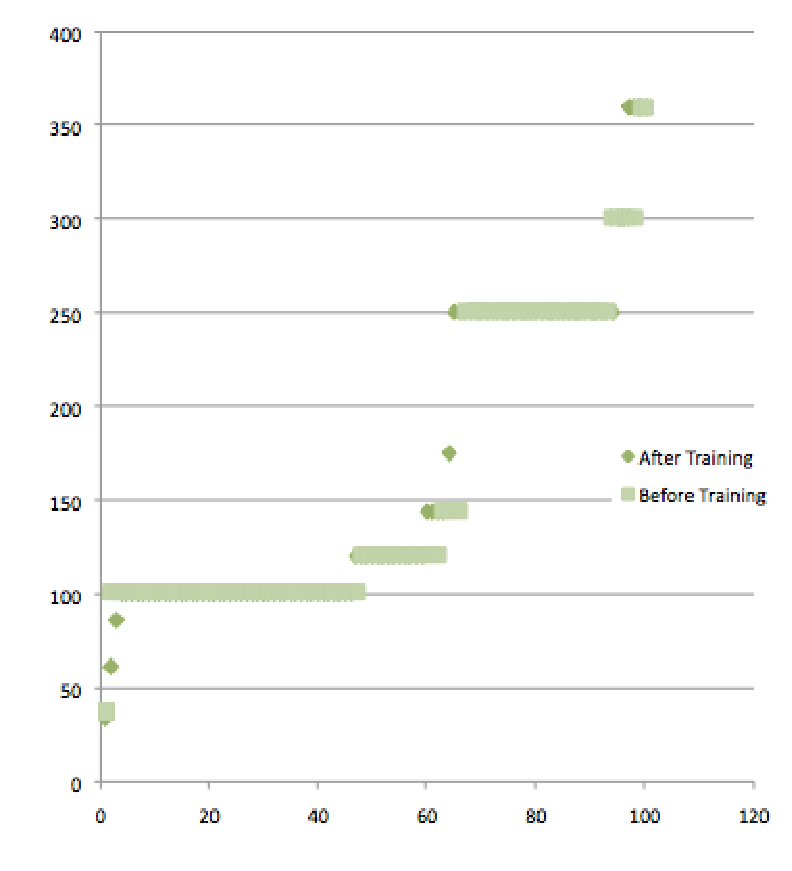
\includegraphics[height=3.5in,width=3.5in]{improved}
\caption{Running Result }
\label{fig:improvedpic}
\end{figure}

To verify our guess, we also can use Kruskal-Wallis rank sum test.  The output shows as following. \\
\begin{table}
\begin{Schunk}
\begin{Sinput}
> kruskal.test(before ~ after, data = airquality)
\end{Sinput}
\begin{Soutput}
	Kruskal-Wallis rank sum test

data:  before by after 
Kruskal-Wallis chi-squared = 96.7472,
 df = 9, p-value < 2.2e-16
\end{Soutput}
\end{Schunk}
\end{table}

From the result, we can see the chi-squred value is close to the $1- \alpha$ value. $\alpha$ traditionally is set to be 0.05.  It means there is no big evidence to see the two samples, before training and after training, are significant different. \\

\subsection{Analysis}
We are not satisfy with the current result. So we have to re-exam our model to see why the improvement is too little to be significant.  \\

\begin{itemize}
\item
The big issue for causing this problem is the unbalanced transition fireup. In the whole running process, we can see certain transitions are triggered during the whole process but with other transitions are in silent.  To rectify this problem, we revised the event generator to make the transition fireup in a chain. However this didn't make up the lack of control on transition firing.  The phenomena still exists and cause problem. \\
\item
The second issue is the entry state change, in actory model, the entries number determines the running time for certain transition. This also would lead to the fire up chain break down.  So another control need to be implemented in the entry point. All these are left for our future work. \\
\end{itemize}

\section{Conclusion and Future work}
In this paper, we proposed a new course planning model established upon actory model.  This course plan model is trying to simulate the students life by mimic real life event.  It implemented under BDI mentalism and fulfilled the requirement of agent programming. However 
this course plan model is still under developing with more features need to be added, such as courses indexing and others.   Also the current concurrent model hardly relies on delay which would cost too much computing time on waiting.?To solve this problem, semaphores or monitor process need to be introduced.  Also we need to improve the learning mechanism to regain much more performance.  For the actory model evolution, there is also some steps need to go.   The idea of role would fulfill the machine have the context awareness capability.   With this view, certain tasks are generated and be assigned to the machine.  This requirement asks for that  the factory should have the capability to create and release machine on demand.   An communication mechanism need to be introduced into actory to fulfill the requirement of communication between machines , machines and factory , and also factory to factory.   In conclude, actory acts as an agent system with an infrastructure of synchronizing information and also grows on demand. 
\newpage
\bibliographystyle{IEEEtran}
\bibliography{sig-alternate}
\end{document}
